\documentclass[11pt,letterpaper]{article}
\usepackage{fullpage}
\usepackage[top=2cm, bottom=4.5cm, left=2.5cm, right=2.5cm]{geometry}
\usepackage{amsmath,amsfonts,amssymb}
\usepackage{lastpage}
\usepackage[inline]{enumitem}
\usepackage{fancyhdr}
\usepackage{mathrsfs}
\usepackage{xcolor}
\usepackage{graphicx}
\usepackage{hyperref}
\usepackage{fancyvrb}
\usepackage[section]{placeins}
\hypersetup{colorlinks=true, linkcolor=blue, linkbordercolor={0 0 1}}

\renewcommand{\arraystretch}{1.75}

\newcommand{\qrf}{\texttt{QRFactor}}

\setlength{\parindent}{0.0in}
\setlength{\parskip}{0.05in}

\pagestyle{fancyplain}
\lhead{Brad Cownden}
\chead{}
\rhead{}
\cfoot{\small\thepage}
\headsep 36pt

\begin{document}

\begin{center}
  {\Large \bf Instructions for Building \texttt{QRFactor}}
\end{center}

This document will outline the settings and libraries required to build and 
execute QRFactor in either Visual Studio (Windows) or a Docker container (Linux). 
It is assumed that \href{https://docs.docker.com/get-docker/}{Docker} and/or 
\href{https://visualstudio.microsoft.com/downloads/}{Microsoft Visual Studio} has 
been installed. If using Visual Studio, the \href{https://developer.nvidia.com/cuda-downloads}{CUDA Toolkit}
will also need to be downloaded separately. If using Docker, a docker account is required
to pull from Docker Hub.
The read-in of the system matrix $A$ requires the data to be in Matrix Market format 
(see the \href{https://math.nist.gov/MatrixMarket/formats.html}{NIST page} for more
information on MMF, as well as to download the library routines \texttt{mmio.h} 
and \texttt{mmio.c}).

\section{Running \texttt{QRFactor} in Visual Studio 2019 (VS2019)}
\label{sec: vs}

Place the system matrix file \texttt{sysMatA.mtx}, the library routines \texttt{mmio.c} and \texttt{mmio.h}, the wrapper \texttt{mmio\_wrapper.cpp}, the source file \texttt{QRFactor.cpp}, and the VS2019 files \texttt{QRFactor.vcxproj} and \texttt{QRFactor.vcxproj.user} in a single directory. The time-dependent input data files can be located in a separate directory that will be set later.

There are several project settings that will need to be changed before the program can be built. These will be discussed below, and screen shots of the relevant settings will be included in appendix~\ref{app: VS settings}. The following settings will ensure that VS2019 is able to find the correct library files:
\begin{itemize}
\item Under Advanced Properties, ensure {\bf MSVC Toolset} is set to 14.25.28610.
\item Under C++/General, ensure {\bf Additional Include Directories} contains ./;\$(CudaToolkitIncludeDir);\$(CudaToolkitIncludeDir)/include;C:/ProgramData/NVIDIA Corporation/CUDA Samples/v10.2/common/inc.
\item Under C++/Optimization, ensure {\bf Optimization} is set to Maximum Optimization (Favour Speed) (/O2).
\item Under Linker/General, ensure {\bf Additional Library Directories} is set to \$(CudaToolitLibDir).
\item Under Linker/Input, ensure {\bf Additional Dependencies} includes cusolver.lib;cusparse.lib; cudart\_static.lib;kernel32.lib;user32.lib;gdi32.lib;winspool.lib;comdlg32.lib;advapi32.lib; \\ shell32.lib;ole32.lib;oleaut32.lib;uuid.lib;odbc32.lib;odbccp32.lib;\%(AdditionalDependencies).
\end{itemize}

With these settings in place, the project can be built by selecting Build $\to$ Build QRFactor (Ctrl + B). \texttt{QRFactor.exe} can then be run either through VS2019 or via the command line.

\section{Running \texttt{QRFactor} in a Docker Container}
\label{sec: docker}

To create the appropriate container, see the instructions in \S~\!\ref{app:docker}. Once again,
the system matrix file \verb+sysMatA.mtx+ -- as well as auxillary files \verb+mmio.c+, \verb+mmio.h+, 
and \verb+mmio_wrapper.cpp+ -- and source file \verb+QRFactor.cpp+ should all be placed in the
same directory. Time-dependent input files can be placed either in the same directory, or in a different directory.

Compilation will take place using a \verb+Makefile+. As a basis, the Makefile provided in the Toolkit sample 
directory \verb+samples/7_CUDALibraries/cuSolverSp_LowlevelQR+ can be copied into the \verb+QRFactor+ directory. The following
changes to that Makefile need to be made:
\begin{itemize}
  \item \verb+ALL_CCFLAGS+ should include an optimization level. To add this, insert a line after \verb+ALL_CCFLAGS:=+ that
  reads \verb.ALL_CCFLAGS+= -O2., or the desired level of optimization.
  \item The location of helper libraries from the CUDA toolkit need to be specified by changing the 
  INCLUDES variable from \verb_INCLUDES:= -I../../common/inc_ to
  \begin{center}
    \verb+INCLUDES:= -I$(CUDA_PATH)/samples/common/inc+
  \end{center} 
  as well as adding an additional line that reads 
  \begin{center}
    \verb.INCLUDES+= -I$(CUDA_PATH)/targets/x86_64-linux/include.
  \end{center} 
  or the equivalent architecture.
\end{itemize}

With these changes to the \verb+Makefile+, the program is compiled by running \verb+make+ as per usual.

%%%%%%%%%%%%%%%%%%%%%%%%%%%%%%%%%%%%%%%%%%%%%%%%%%%%%%%%%%%%%%%%%%%%%%%%%%%%%%
%%%%%%%%%%%%%%%%%%%%%%%%%%%%%%%%%%%%%%%%%%%%%%%%%%%%%%%%%%%%%%%%%%%%%%%%%%%%%%

\appendix

\section{Visual Studio Settings}
\label{app: VS settings}

Included below are screen shots of the options discussed in \S~\!\ref{sec: vs} for
running \verb+QRFactor+ in VS2019.

\begin{figure}[!h]
  \centering
  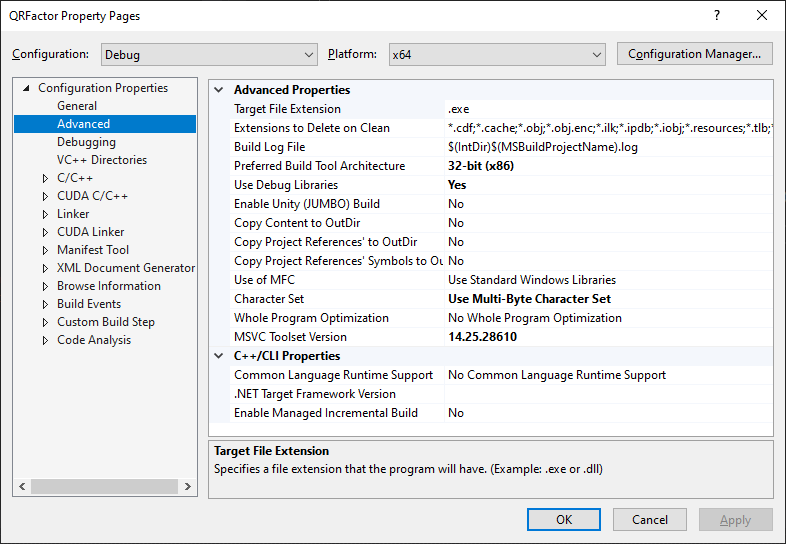
\includegraphics[width=0.75\textwidth]{C:/Users/bradc/Documents/MHI/Reports/ConfigProperties_Advanced}
  \label{f: configproperties_advanced}
  \caption{QRFactor Properties $\to$ Advanced}
\end{figure}

\begin{figure}[!h]
  \centering
  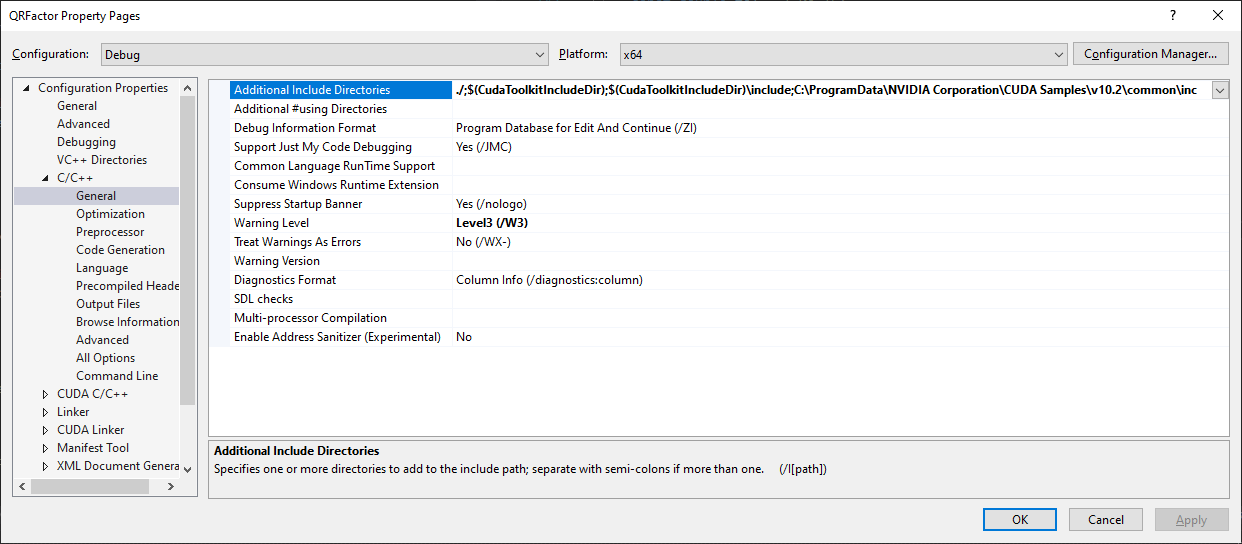
\includegraphics[width=0.9\textwidth]{C:/Users/bradc/Documents/MHI/Reports/CplusplusProperites_General}
  \caption{QRFactor Properties $\to$ C/C$++$ $\to$ General}
\end{figure}

\begin{figure}[!h]
  \centering
  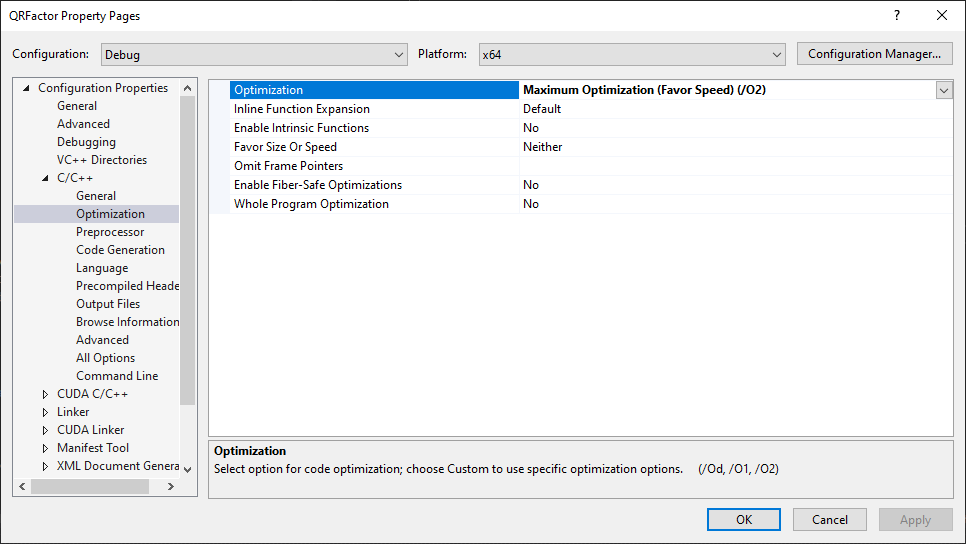
\includegraphics[width=0.9\textwidth]{C:/Users/bradc/Documents/MHI/Reports/CplusplusProperites_Optimization}
  \caption{QRFactor Properties $\to$ C/C$++$ $\to$ Optimization}
\end{figure}

\begin{figure}[!h]
  \centering
  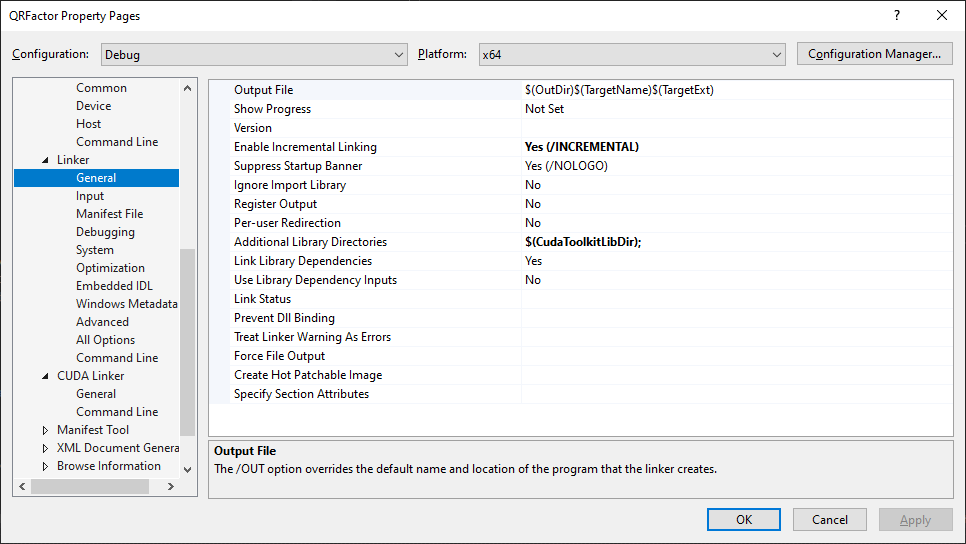
\includegraphics[width=0.9\textwidth]{C:/Users/bradc/Documents/MHI/Reports/Linker_General}
  \caption{QRFactor Properties $\to$ Linker $\to$ General}
\end{figure}

\begin{figure}[!h]
  \centering
  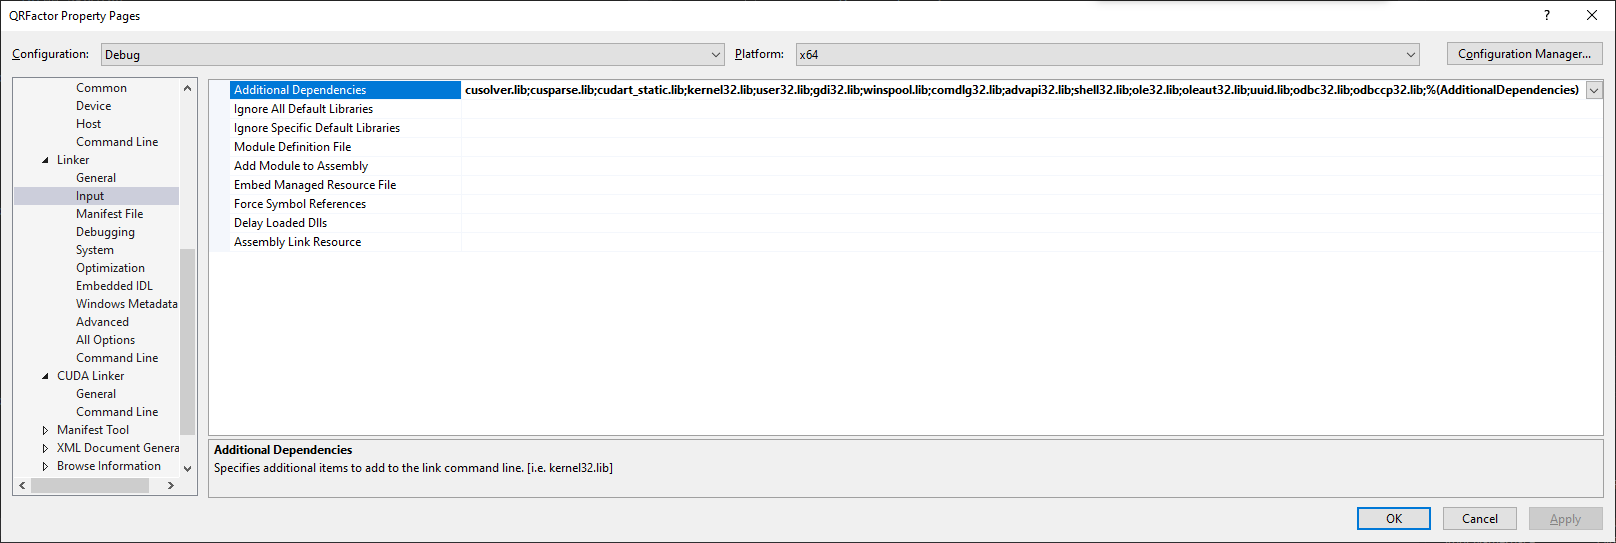
\includegraphics[width=\textwidth]{C:/Users/bradc/Documents/MHI/Reports/Linker_Input}
  \caption{QRFactor Properties $\to$ Linker $\to$ Input}
\end{figure}

%%%%%%%%%%%%%%%%%%%%%%%%%%%%%%%%%%%%%%%%%%%%%%%%%%%%%%%%%%%%%%%%%%%%%%%%%%%%%%

\section{Docker}
\label{app:docker}

Included below are the steps required to create a custom CUDA image that includes
the CUDA Toolkit within a linux-based Docker container. Also included are sample commands for running
a container based on that image.

\begin{enumerate}
  \item In the desired directory, create a file named `Dockerfile' with no extension. This file
  will include instructions for creating an image that will provide the basis for the development
  environment. The Dockerfile is provided in \S~\!\ref{app:dockerfile}. To make the image, run
  \begin{center}
    \verb+docker build -t <CUDA_IMAGE> .+
  \end{center}
  where \verb+<CUDA_IMAGE>+ is the name chosen for the image that is being created.
  \item Allow Docker to run through the steps involved in creating the image -- this should not require
  any input from the user. This process can also be lengthly, but will only need to happen once.
  \item Confirm the image has been created by running \verb+docker images ls+ and confirming that
  \verb+<CUDA_IMAGE>+ was created. 
  \item Edit the contents of \texttt{runCUDA.sh} (provided in \S~\!\ref{app:runcuda}) to set \verb+<CUDA_IMAGE>+ to the image that
  was just created, and \verb+<CUDA_CONTAINER>+ to the name chosen for the container that development
  will occur within. Volumes can be mapped into/out of the container using the \texttt{-v} option, as shown. Running 
  \texttt{bash runCUDA.sh} will create and enter \verb+<CUDA_CONTAINER>+.
  \item The container can be exited without stopping by pressing \texttt{Ctrl+q, Ctrl+p} and reentered 
  later by running \verb+docker attach <CUDA_CONTAINER>+.
  \item To perminantly delete the container or image, run \verb+docker rm <CUDA_CONTAINER>+
  or \\\verb+docker rmi <CUDA_IMAGE>+.
\end{enumerate}



%%%%%%%%%%%%%%%%%%%%%%%%%%%%%%%%%%%%%%%%%%%%%%%%%%%%%%%%%%%%%%%%%%%%%%%%%%%%%%

\section{\texttt{Dockerfile}}
\label{app:dockerfile}

\begin{verbatim}
FROM nvidia/cuda:10.2-base-ubuntu18.04
 
# Package management functions 
RUN apt-get update 
RUN apt-get install -y apt-utils && \
apt-get install -y wget && \
apt-get install -y gnupg && \
apt-get install -y curl && \
apt-get install -y linux-headers-$(uname -r) 

# Get CUDA Toolkit (see https://docs.nvidia.com/cuda/cuda-installation-guide-linux/index.html)
RUN wget https://developer.download.nvidia.com/compute/cuda/
                                        repos/ubuntu1804/x86_64/cuda-ubuntu1804.pin
RUN mv cuda-ubuntu1804.pin /etc/apt/preferences.d/cuda-repository-pin-600 
RUN wget http://developer.download.nvidia.com/compute/cuda/10.2/Prod/local_installers/
                  cuda-repo-ubuntu1804-10-2-local-10.2.89-440.33.01_1.0-1_amd64.deb
RUN dpkg -i cuda-repo-ubuntu1804-10-2-local-10.2.89-440.33.01_1.0-1_amd64.deb 
RUN apt-key add /var/cuda-repo-10-2-local-10.2.89-440.33.01/7fa2af80.pub 
RUN apt-get update 
RUN DEBIAN_FRONTEND=noninteractive apt-get install -y cuda

# Install samples that can be executed
RUN cuda-install-samples-10.2.sh /home/cuda-samples

# Clean
RUN apt-get clean && rm -rf /var/lib/apt/lists/* /temp/* /var/temp/* 

# Update PATHs
RUN export PATH=/usr/local/cuda-10.2/bin:/usr/local/cuda-10.2/
                                                  NsightCompute-2019.1${PATH:+:${PATH}}
RUN export LD_LIBRARY_PATH=/usr/local/cuda-10.2/lib64${LD_LIBRARY_PATH:+:${LD_LIBRARY_PATH}}
\end{verbatim}

\section{\texttt{runCUDA.sh}}
\label{app:runcuda}

\begin{verbatim}
# Run a docker container with cuda installed and gpus active
docker run -it --gpus all \
#    -v /home/bradc/MHI/Upload:/home/data \
#    -v /home/bradc/MHI/QRFactor:/home/QRFactor \
     --name <CUDA_CONTAINER> \
    <CUDA_IMAGE>
\end{verbatim}

























\end{document}
